\documentclass{beamer}

\usepackage{graphicx}
\usepackage{caption}
\usepackage{subcaption}

\title{Einbindung von Constraints in eine divergente Optimierungsmethode am Beispiel der Surrogat-assistierten Illumination} 
\author[Jan Kruska]{Jan Kruska}
\date{28.02.2020}

%
%    \setbeamertemplate{footline}{%
%	\raisebox{5pt}{\makebox[\paperwidth]{\hfill\makebox[10pt]{\scriptsize\insertframenumber/\inserttotalframenumber}}}}

\setbeamertemplate{frametitle}{\nointerlineskip  
	\begin{beamercolorbox}[wd=\paperwidth,ht=2.75ex,dp=1.375ex]{frametitle}
		\hspace*{2ex}\insertframetitle \hfill {\scriptsize\insertframenumber/\inserttotalframenumber} \hspace*{1ex}%
	\end{beamercolorbox}}

\begin{document}

\begin{frame}{}
	\titlepage
\end{frame}

\frame{\tableofcontents}

\section{Radkästen}
\subsection{Problem}
\frame{\frametitle{Problem}
	\begin{block}{Problem}
		Die Radkästen des Velomobils beschränken den maximal möglichen Radausschlag
	\end{block}
	\begin{itemize}
		\item Generierung von Radkästen die aerodynamisch gut sind und trotzdem den maximalen Radausschlag ermöglichen 
	\end{itemize}
}
\note[itemize]{
	divergent, surrogatassistenz
}
\subsection{Methode}
\frame{\frametitle{SAIL}
\begin{figure}
	\centering
	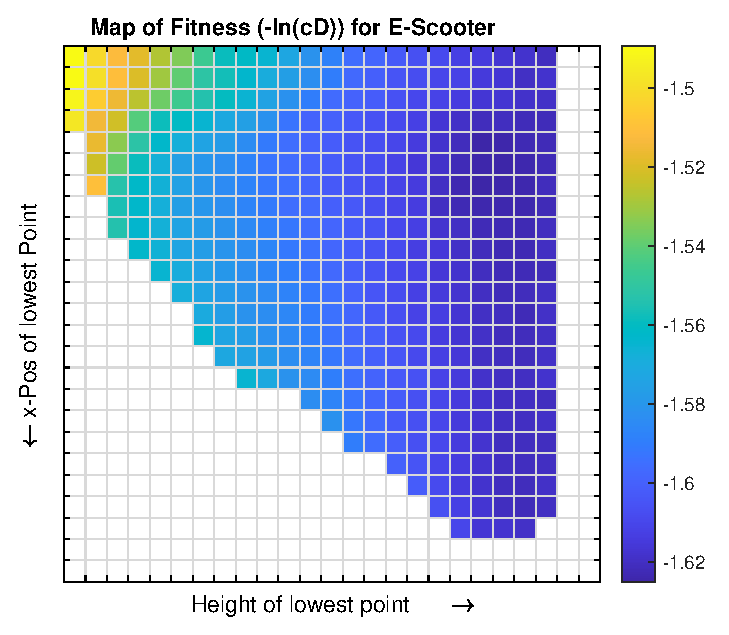
\includegraphics[width=.7\linewidth]{../thesis/bilder/escooter/dragMapEscooter}
\end{figure}

}
\frame{\frametitle{Freiformdeformation}
	\begin{figure}[h]
		\centering
		\begin{minipage}{0.45\textwidth}
			\centering
			\includegraphics[width=1\linewidth]{../thesis/bilder/sphere_lattice}
%			\caption{3D-Mesh einer Kugel in 4x4x4 FFD-Box}
			\label{fig:ffd_undeformed}
		\end{minipage}\hfill
		\begin{minipage}{0.45\textwidth}
			\centering
			\includegraphics[width=1\linewidth]{../thesis/bilder/sphere_lattice_deformed2}
%			\caption{Deformiertes 3D-Mesh ezeugt durch Bewegung der Deformationspunkte}
			\label{fig:ffd_deformed}
		\end{minipage}
	\end{figure}
}
\frame{\frametitle{FFD-Konfiguration}
	\begin{figure}
		\centering
		\includegraphics[width=.7\linewidth]{../thesis/bilder/6ptDeformationPoints.png}
	\end{figure}
}
\frame{\frametitle{Features}
	\begin{itemize}
		\item MAP-Elites benötigt Kategorien an denen die Karte aufgeteilt wird
		\item Die Kategorien sind:
		\begin{enumerate}
			\item Breite des Velomobils/Radkastens
			\item x-Position des breitesten Punkts\footnote{Das Velomobil zeigt in -X-Richtung}
		\end{enumerate}
		\item Hypothesen
		\begin{enumerate}
			\item Breitere Velomobile weisen einen stärkeren Luftwiderstand auf
			\item Breitere Velomobile erfüllen eher den Constraint
		\end{enumerate}
	\end{itemize}
}

\frame{\frametitle{Soft Constraint vs. Hard Constraint}
	\begin{itemize}
		\item Zwei, den Constraint verletzende, Lösungen können sich in der Stärke der Verletzung unterscheiden
		\item Der Ausgangsradkasten erfüllt den Constraint nicht, es sind also keine nicht-triviale erfüllende Bauteile bekannt.
		\item[$\Rightarrow$] Soft Constraint besser geeignet
	\end{itemize}
}

\frame{\frametitle{Radausschlagsvolumen}
	Alle mögliche Radausschläge können als Volumen wie folgt modelliert werden:
	\begin{figure}
		\includegraphics[width=1\linewidth]{../thesis/bilder/radausschlag.png}
	\end{figure}
}

\frame{\frametitle{Constraint + Velomobil}
	Es ist gut erkennbar, dass der Ausgangsradkasten den Constraint verletzt 
	\begin{figure}
		\includegraphics[width=1\linewidth]{../thesis/bilder/radausschlag_inclVelo.png}
	\end{figure}
}

\frame{\frametitle{Constraint Volume}
	Zur Berechnung des Constraint wird die Meshdifferenz von Radauschlagsvolumen und Radkasten gebildet und deren Volumen berechnet
	\begin{figure}
		\includegraphics[width=1\linewidth]{../thesis/bilder/difference.png}
	\end{figure}
	Diese Volumen entspricht zwar nicht vollständig dem Constraint, generell wird angenommen, dass eine Reduzierung des Volumens zu einer Verbesserung des Constraints führt.
}

\subsection{Ergebnisse}
\frame{\frametitle{SAIL-Parameter}
	\begin{enumerate}
		\item Reale Funktionsauswertungen: 1000
		\item Akquisegenerationen: 2048
		\item Ergebnisgenerationen: 8192
		\item Kinder pro Generation : 32
		\item Kartenauflösung: 25x25
	\end{enumerate}
}

\frame{\frametitle{Comparison non-constrained vs. constrained}
	\vspace*{\fill}
\begin{figure}[h]
	\centering
	\begin{minipage}{0.45\textwidth}
		\centering
		\includegraphics[width=1\linewidth]{../thesis/bilder/6pt1000Samples/dragBoxplot}
%		\caption{Comparison of final drag values}
		\label{fig:3rddragbox}
	\end{minipage}\hfill
	\begin{minipage}{0.45\textwidth}
		\centering
		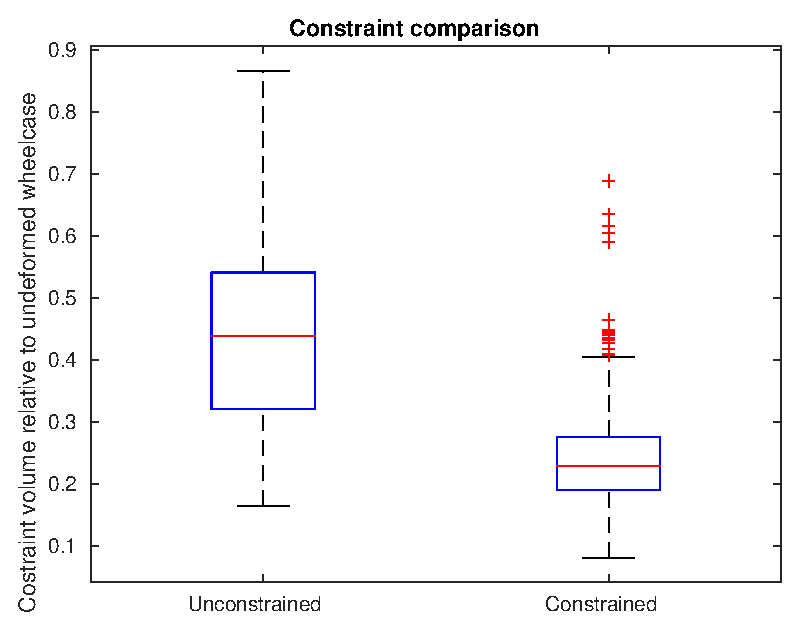
\includegraphics[width=1\linewidth]{../thesis/bilder/6pt1000Samples/constraintBoxplot}
%		\caption{Comparison of final constraint values}
		\label{fig:3rdconbox}
	\end{minipage}
\end{figure}
}

\frame{\frametitle{Luftwiderstandskarten}
\begin{figure}[h]
	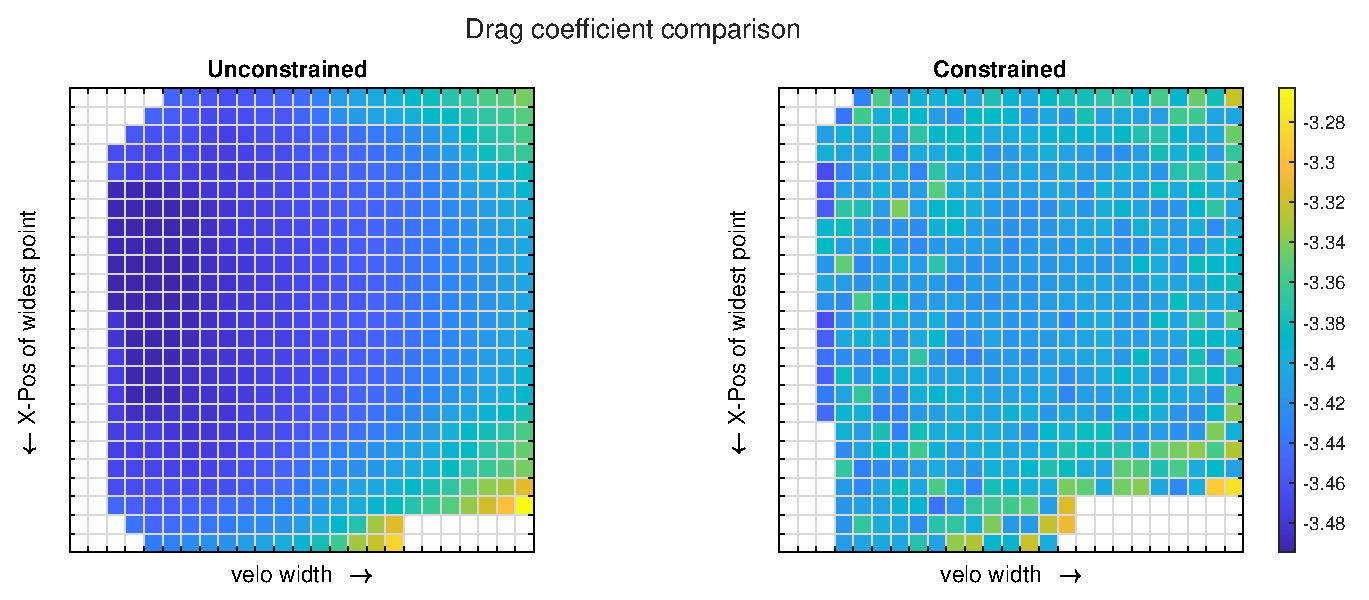
\includegraphics[width=1\linewidth]{../thesis/bilder/6pt1000Samples/dragMapComparison}
%	\caption{Maps of final drag values}
	\label{fig:3rdmapDrag}
\end{figure}
}

\frame{\frametitle{Luftwiderstand gegen Spalten}

\begin{figure}[h]
	\centering
	\begin{subfigure}[t]{0.5\textwidth}
		\centering
		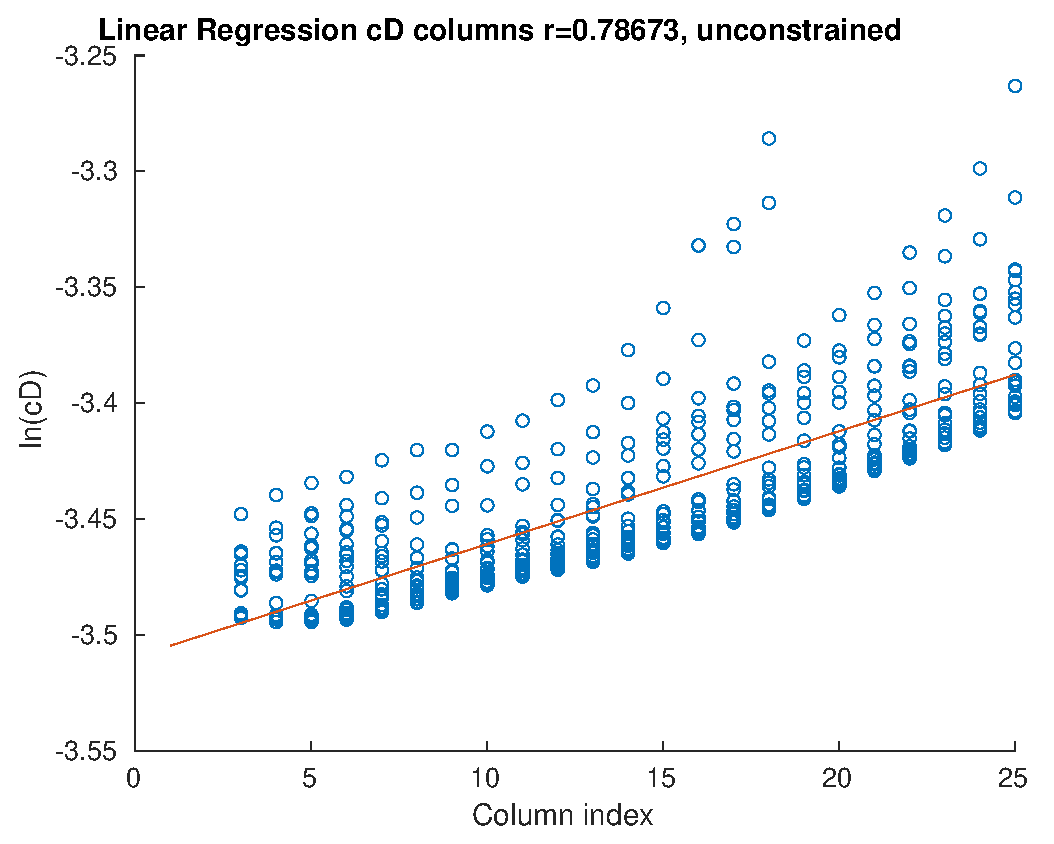
\includegraphics[width=1\linewidth]{../thesis/bilder/6pt1000Samples/cDRegressionUncon}
	\end{subfigure}\hfill
	\begin{subfigure}[t]{0.5\textwidth}
		\centering
		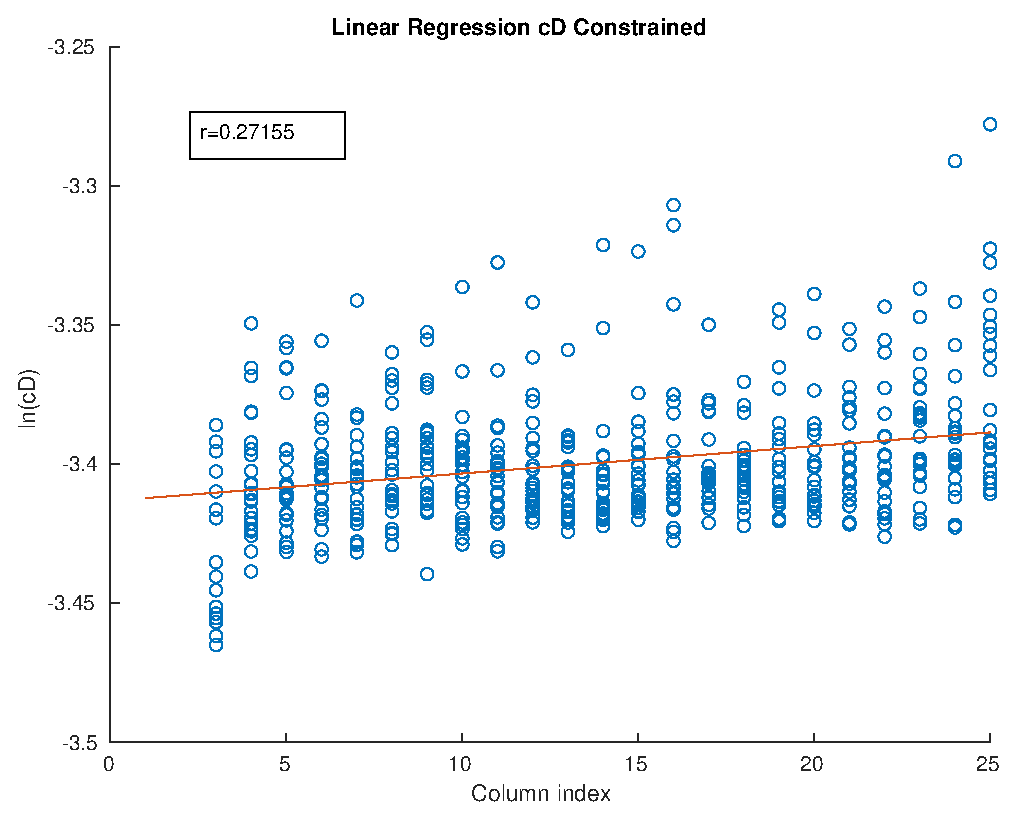
\includegraphics[width=1\linewidth]{../thesis/bilder/6pt1000Samples/cDRegressionCon}
	\end{subfigure}
	\label{fig:regCDCol}
\end{figure}
}

\frame{\frametitle{Luftwiderstand gegen Zeilen}
\begin{figure}[h]
	\centering
	\begin{subfigure}[t]{0.5\textwidth}
		\centering
		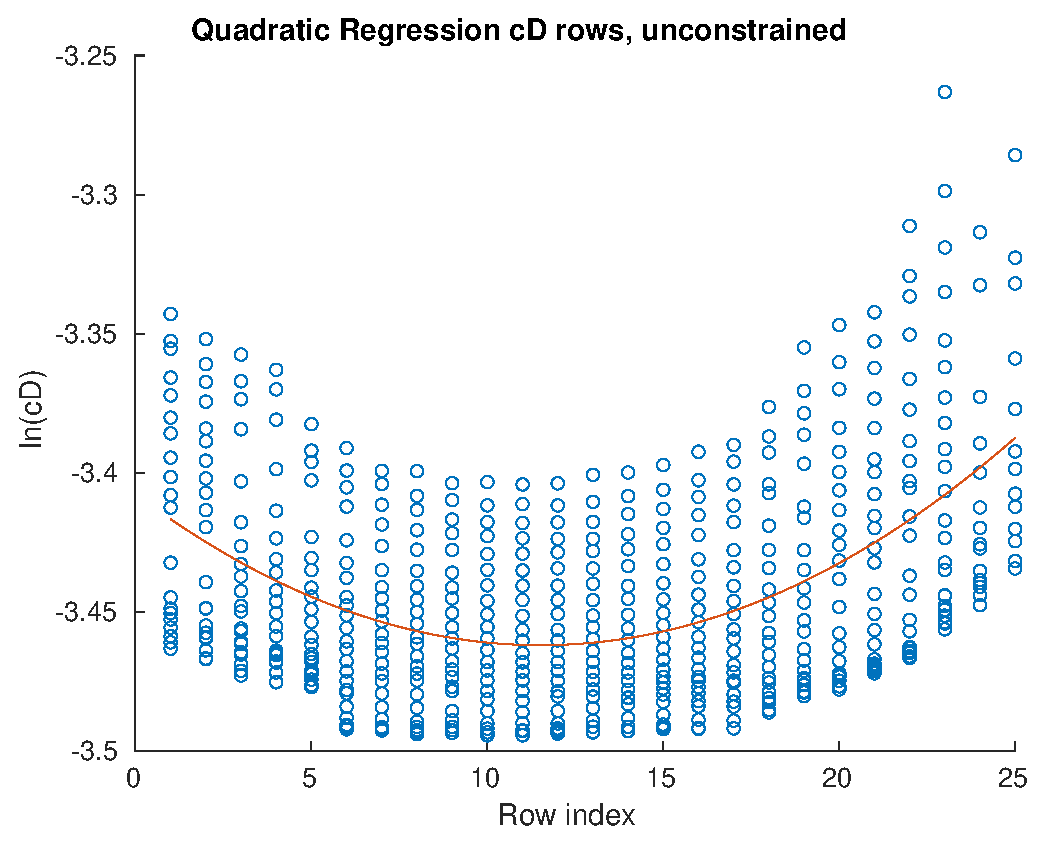
\includegraphics[width=1\linewidth]{../thesis/bilder/6pt1000Samples/cDRegressionRowUncon}
	\end{subfigure}\hfill
	\begin{subfigure}[t]{0.5\textwidth}
		\centering
		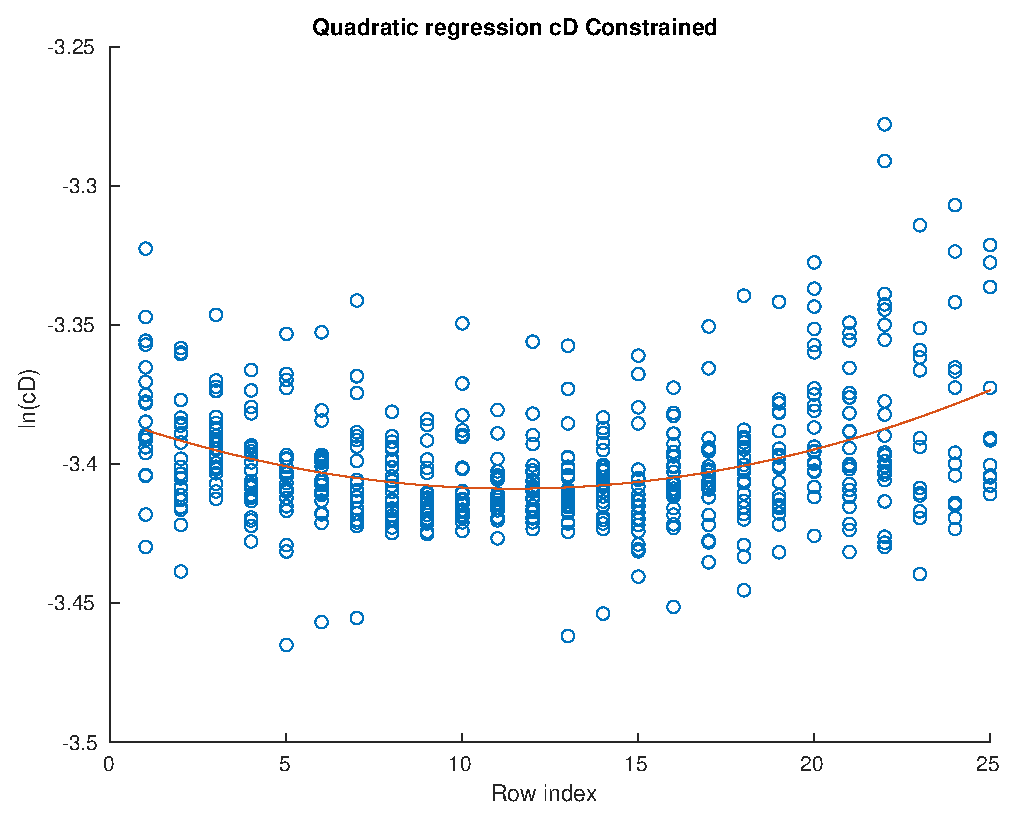
\includegraphics[width=1\linewidth]{../thesis/bilder/6pt1000Samples/cDRegressionRowCon}
	\end{subfigure}
	\label{fig:regCDRow}
\end{figure}}

\frame{\frametitle{Constraintkarten}
	\begin{figure}[h]
		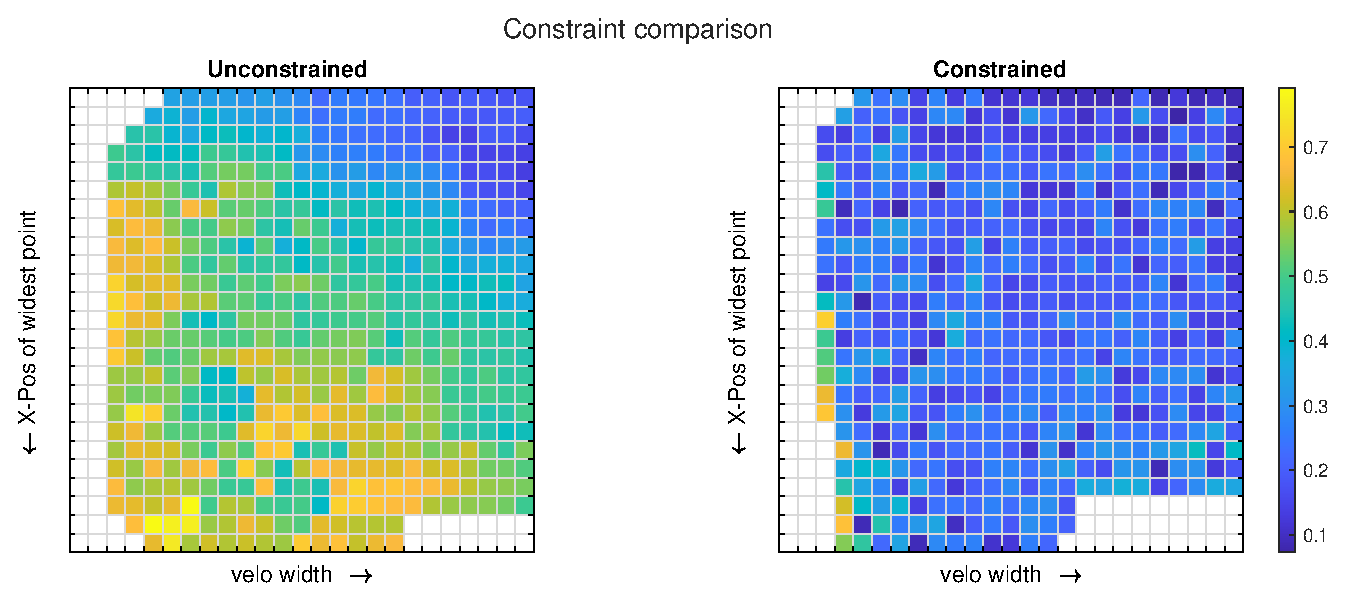
\includegraphics[width=1\linewidth]{../thesis/bilder/6pt1000Samples/constraintMapComparison}
%		\caption{Maps of final constraint values}
		\label{fig:3rdmapCon}
	\end{figure}
}

\frame{\frametitle{Constraint gegen Spalten}
\begin{figure}[h]
	\centering
	\begin{subfigure}[t]{0.5\textwidth}
		\centering
		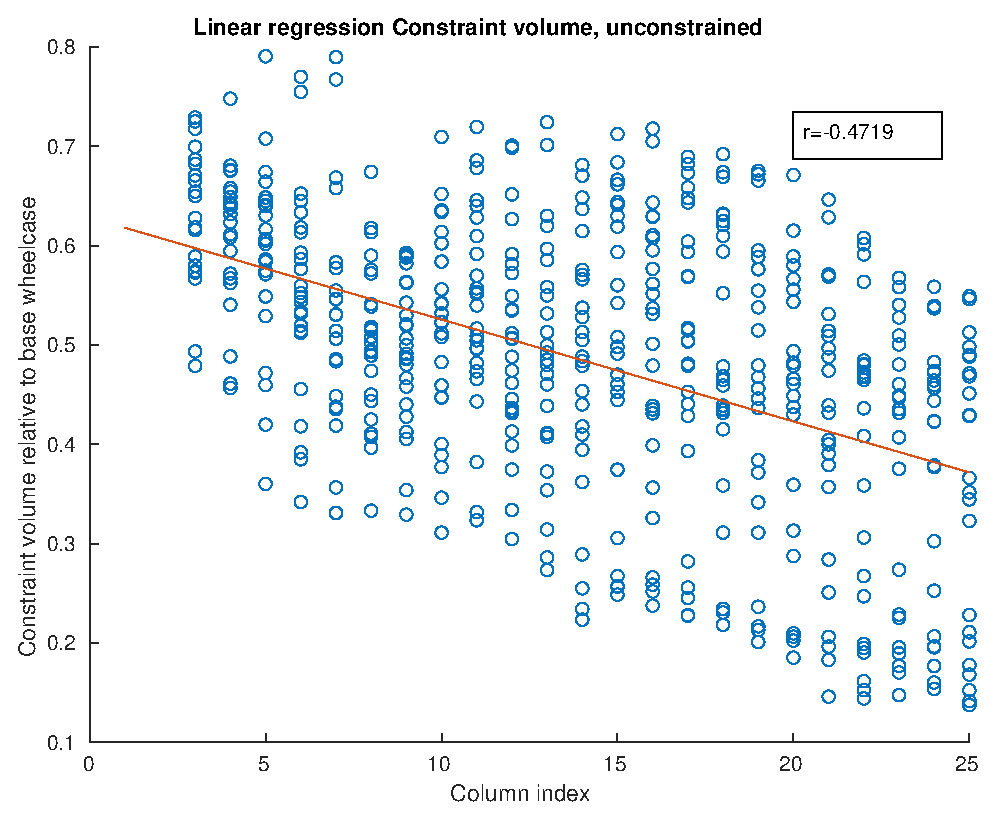
\includegraphics[width=1\linewidth]{../thesis/bilder/6pt1000Samples/conRegressionUnconCol}
	\end{subfigure}\hfill
	\begin{subfigure}[t]{0.5\textwidth}
		\centering
		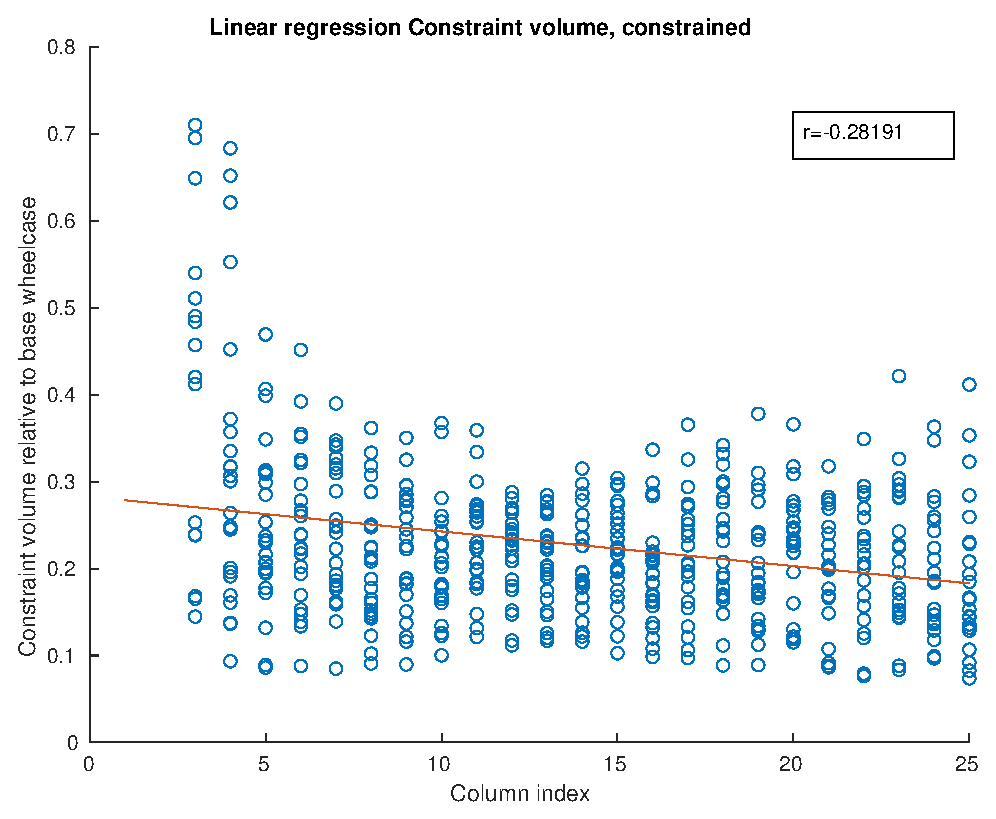
\includegraphics[width=1\linewidth]{../thesis/bilder/6pt1000Samples/conRegressionConCol}
	\end{subfigure}
	\label{fig:regConCol}
\end{figure}
}

\newcommand{\wheelcasepheno}[3]{
	\begin{figure}[h]
		\centering
		\begin{subfigure}[t]{0.5\textwidth}
			\centering
			\includegraphics[width=1\linewidth]{../thesis/bilder/6pt1000Samples/#1-uncon-top.png}
			\subcaption{oben, ohne Constraint, $c_D$=#2}
		\end{subfigure}\hfill
		\begin{subfigure}[t]{0.5\textwidth}
			\centering
			\includegraphics[width=1\linewidth]{../thesis/bilder/6pt1000Samples/#1-uncon-angled.png}
			\subcaption{perspektivisch, ohne Constraint}
		\end{subfigure}
		\begin{subfigure}[b]{0.5\textwidth}
			\centering
			\includegraphics[width=1\linewidth]{../thesis/bilder/6pt1000Samples/#1-con-top.png}
			\subcaption{oben, mit Constraint, $c_D$=#3}
		\end{subfigure}\hfill
		\begin{subfigure}[b]{0.5\textwidth}
			\centering
			\includegraphics[width=1\linewidth]{../thesis/bilder/6pt1000Samples/#1-con-angled.png}
			\subcaption{perspektivisch, mit Constraint}
		\end{subfigure}
		\label{fig:wheelcasepheno#1}
	\end{figure}
}

%\newcommand{\allrefWheelcase}[1]{
%	\cref{\wref{#1}{uncon-top},\wref{#1}{uncon-angled},\wref{#1}{con-top},\wref{#1}{con-angled}}
%}

\frame{\frametitle{Schmales Individuum (4,3)}
\wheelcasepheno{4-3}{0,0315}{0,0336}
}

%\wheelcasepheno{4-24}{0,0321}{0,0327}

\frame{\frametitle{Breites Individuum (25,22)}
	\wheelcasepheno{25-22}{0,0365}{0,0377}
}

\frame{\frametitle{Ausgeglichenes Individuum (12,12)}
\wheelcasepheno{12-12}{0,0311}{0,0327}
}

\frame{\frametitle{Diskussion}
	\begin{itemize}
		\item cD Werte in der Version mit Constraint schlechter, das war zu erwarten
		\item Hauptgewinne bei zentraleren Individuen
		\item x-Deformationen scheinen weitestgehend unwichtig zu sein
	\end{itemize}
}
\subsection{Ausblick}
\frame{\frametitle{Ausblick}
	\begin{itemize}
		\item Freiheitsgrade
		\begin{itemize}
			\item Weitere Erhöhung
			\item Keine Deformationen in x
			\item Deformationen in z nur in oberer/unterer Reihe
		\end{itemize}
		\item Constraint als Feature aufnehmen, dadurch Diversität über den Constraint
		\item Automatic relevance determination in Kovarianzfunktion
	\end{itemize}
}
%\section{Future experiments}
%\frame{\frametitle{Future changes}
%\begin{itemize}
%	\item Change FFD-parameters, to facilitate more degrees of freedom
%	\item Longer rund, more generations \& more OpenFoam Evaluations
%\end{itemize}
%}

\section{E-Roller}
\subsection{Methode}
\frame{\frametitle{Bauteil}
	\begin{figure}
		\centering
		\includegraphics[width=\linewidth]{../thesis/bilder/escooter_component}
	\end{figure}
}

\frame{\frametitle{FFD-Configuration}
	\begin{figure}
		\centering
		\includegraphics[width=\linewidth]{../thesis/bilder/escooter_deformationPoints}
	\end{figure}
}
\frame{\frametitle{Features}
	\begin{itemize}
		\item MAP-Elites benötigt Kategorien an denen die Karte aufgeteilt wird
		\item Die Kategorien sind:
		\begin{enumerate}
			\item Höhe des tiefsten Punkts des Bauteils
			\item x-Position des tiefsten Punkts\footnote{Der E-Roller zeigt in -X-Richtung}
		\end{enumerate}
	\end{itemize}
}

\frame{\frametitle{SAIL-Parameters}
	\begin{enumerate}
		\item Real Evaluations: 500
		\item Generations Acquisition: 2048
		\item Generations result: 4096
		\item Children per Gen : 32
		\item Map-resolution: 25x25
	\end{enumerate}
}
\subsection{Ergebnisse}
\frame{\frametitle{$c_D$-Karte in der E-Roller-Domäne}
\begin{figure}[h]
	\centering
	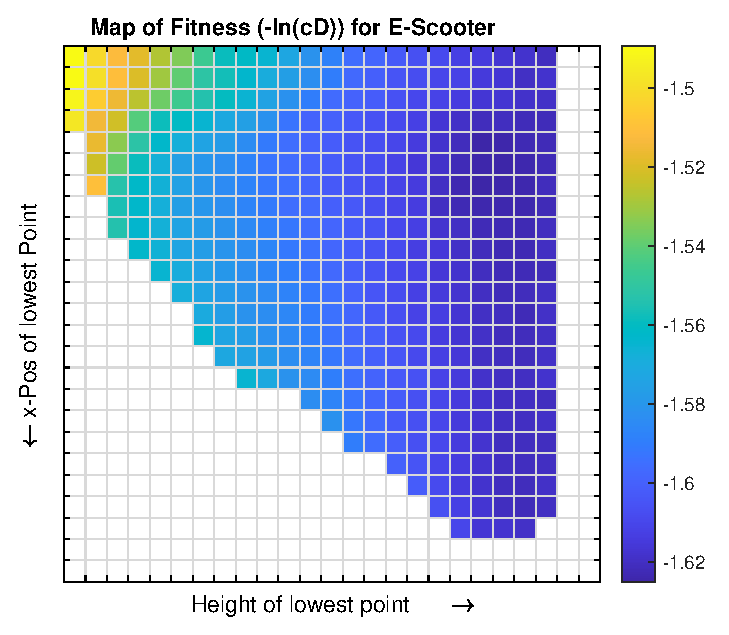
\includegraphics[width=.7\linewidth]{../thesis/bilder/escooter/dragMapEscooter}
	\label{fig:dragMapEscooter}
\end{figure}
}

\newcommand{\escooterpheno}[2]{
	\begin{figure}[h]
		\centering
		\begin{subfigure}[t]{0.5\textwidth}
			\centering
			\includegraphics[width=1\linewidth]{../thesis/bilder/escooter/#1-front.png}
			\subcaption{vorne}
			%		\label{fig:escooterpheno#1-front}
		\end{subfigure}\hfill
		\begin{subfigure}[t]{0.5\textwidth}
			\centering
			\includegraphics[width=1\linewidth]{../thesis/bilder/escooter/#1-side.png}
			\subcaption{Seite}
			%		\label{fig:escooterpheno#1-side}
		\end{subfigure}
%		\caption{Die Phänotypen des Individuums (#1), $c_D$=#2}
		\label{fig:escooterpheno#1}
	\end{figure}
}
\frame{\frametitle{Oben links}
	\escooterpheno{1-1}{0,2255}
}
\frame{\frametitle{Unten rechts}
	\escooterpheno{23-22}{0,1979}
}
\frame{\frametitle{Auf Dreiecksfront}
	\escooterpheno{9-16}{0,2091}
}

\subsection{Probleme \& Ausblick}
\frame{\frametitle{Konvergenz der Openfoam-Simulation}
	\begin{figure}[h]
		\centering
		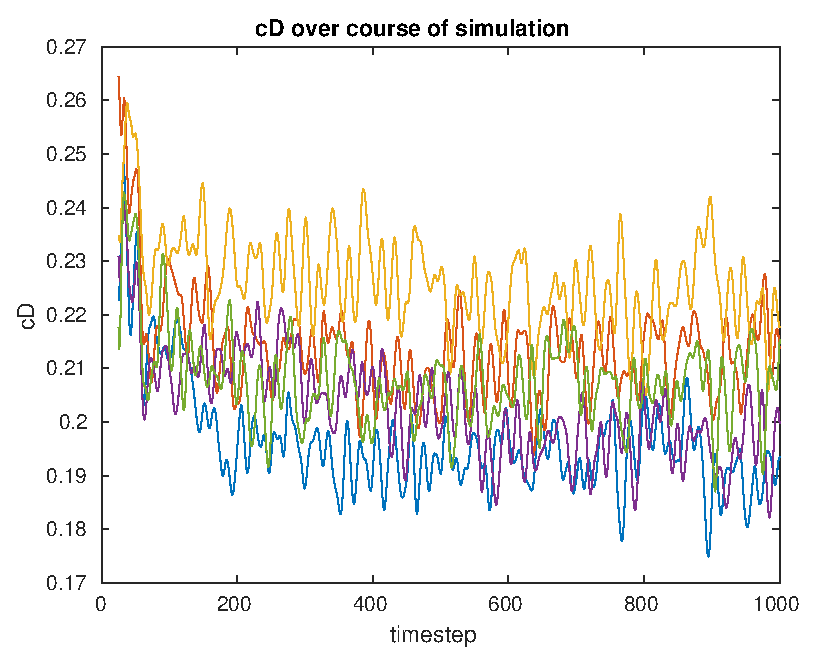
\includegraphics[width=.7\linewidth]{../thesis/bilder/escooterCDConvergence}
	\end{figure}
}

\frame{\frametitle{Laufzeit der Openfoam-Simulation}
	\begin{figure}[h]
		\centering
		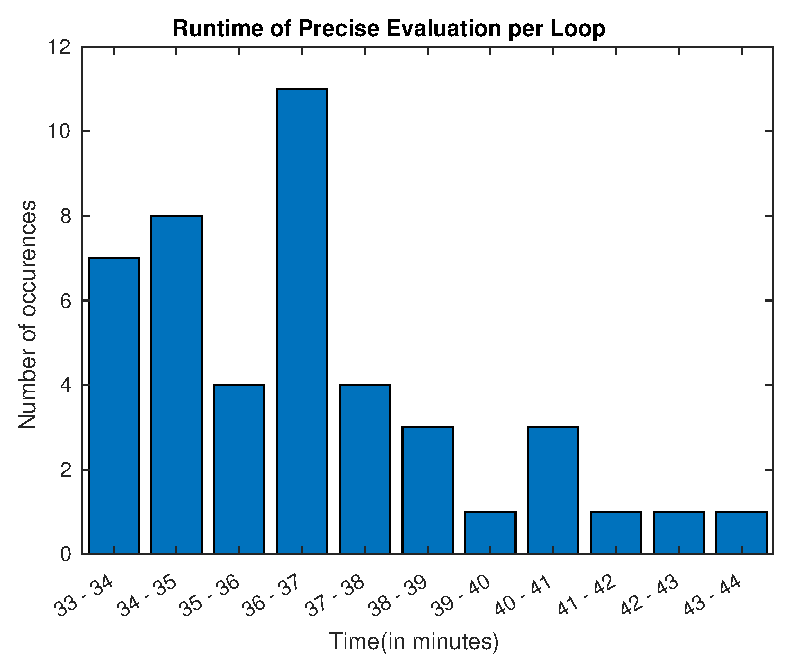
\includegraphics[width=.7\linewidth]{../thesis/bilder/escooter/peRuntime}
	\end{figure}
}

\end{document}
